\section{
    Implemente no JFlap uma MT que reconheça a seguinte linguagem: \{cadeias binárias que não contenham a subcadeia 101\}
    }

\setlength{\parindent}{4em}
\setlength{\parskip}{0.5em}
\renewcommand{\baselinestretch}{1}

\begin{figure}[h]
    \centering
    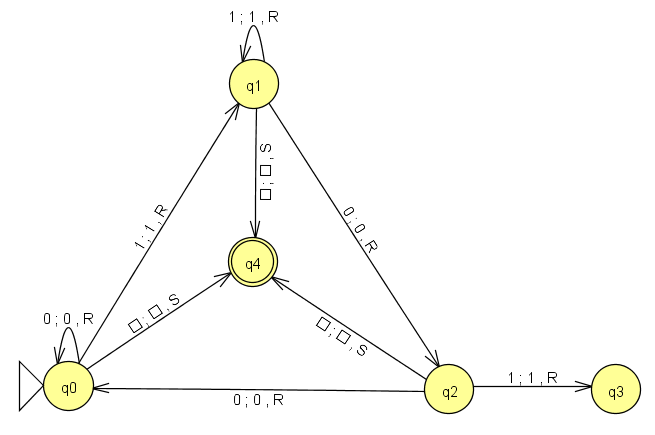
\includegraphics[width=0.65\textwidth]{mtex3.png}
    \caption{Máquina de Turing desenvolvida para o exercício no JFlap.}
    \label{fig:mtex3}
\end{figure}

A máquina de Turing desenvolvida é de fita simples e faz uma leitura sequencial da cadeia inserida na fita. Ela funciona da seguinte forma:
\begin{itemize}
    \item A ideia é que se houver a subcadeia \(101\) na cadeia de entrada, ela vai chegar no estado \(q3\) que não tem nenhuma transição. Uma vez nesse estado ela vai rejeitar a cadeia de entrada independente do que venha depois.

    \item  Ao ler um espaço sem símbolos a máquina entende que a cadeia finalizou e, se estiver em qualquer um dos estados \{\(q0, q1, q3\)\}, ela vai para o estado final \(q4\), que conclui a leitura e aceita a cadeia de entrada. 
\end{itemize}

O arquivo do JFlap com a implementação da Máquina de Turing está em anexo, nomeada \textit{ex3.jff}.
